\pdfminorversion=4
\documentclass[]{article}
\usepackage[utf8]{inputenc}
\usepackage{amssymb,latexsym,amsmath}
\usepackage[a4paper,top=3cm,bottom=2cm,left=3cm,right=3cm,marginparwidth=1.75cm]{geometry}
\usepackage{graphicx}
\usepackage[colorlinks=true, allcolors=blue]{hyperref}
\begin{document}

\title{RPC File Transfer Protocol}
\author{Dinh Khanh Minh Bi12-265}
\date{\today}

\maketitle

\tableofcontents
\newpage

\section{Introduction}
\subsection{Overview}
\noindent%
In this labwork, I try to build a file transfer using RPC. This labwork will be written in C.

\subsection{Protocol}

\begin{figure}[h]
    \centering
    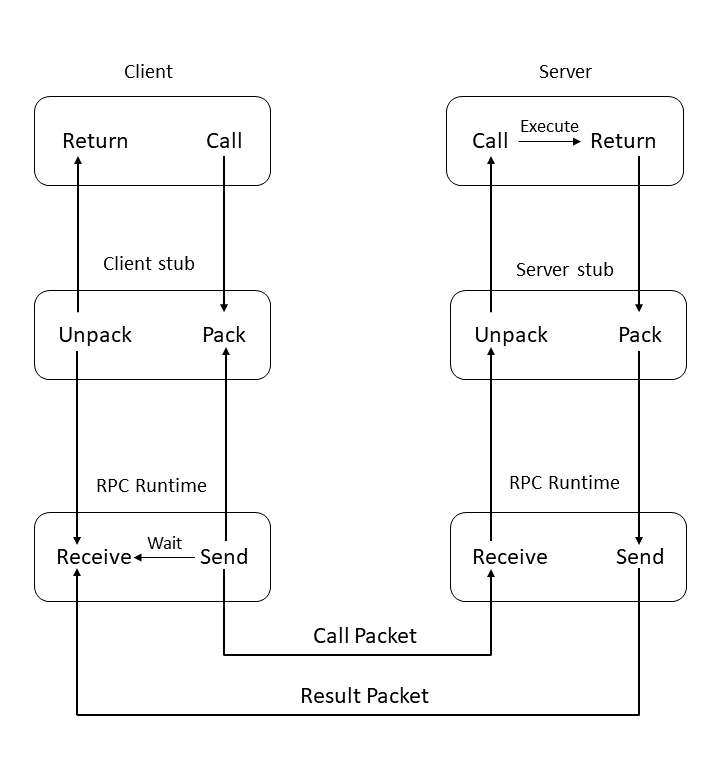
\includegraphics[scale=0.5]{images/RPC.png}
    \caption{Protocol diagram}
    \label{fig:protocol}
\end{figure}

\begin{itemize}
    \item The client calls the client stub, which is a local procedure call.
    \item The client stub packs the parameters into a message and makes a system call to send the message.
    \item The client's local operating system sends the message from the client machine to the server machine.
    \item The local operating system on the server machine passes the incoming packets to the server stub.
    \item The server stub unpacks the parameters from the message. 
    \item Finally, the server stub calls the server procedure.
\end{itemize}

\subsection{System organization}
\noindent%
Through UDP, the client and the server will be connected.

\begin{figure}[H]
    \centering
    \includegraphics[scale=1.0]{images/system.png}
    \caption{System organization}
\end{figure}

\subsection{Implementation}
\noindent%
At first, I created a file a named it file.x. The code was implimented as follows:
\begin{minted}{c}
const MAX_SIZE = 1024;
struct file{
    char filename[MAX_SIZE];
    char buffer[MAX_SIZE];
    int buffer_size;
};

program FILESTRANSFER {
	version FILESTRANSFER_1 {
		int transfer_file(file)=1;
	} = 1;
} = 0x31230000;
\end{minted}

\noindent%
Client and server stubs were generated when I typed "rpcgen -a -C file.x".

\noindent%
I have implemented the client side:

\begin{minted}[linenos,tabsize=2,breaklines]{c}
#include "file.h"
#include <time.h>

void filestransfer_1(char* host, char* filename)
{
	CLIENT* clnt;
	FILE* fp;
	int* result_1;
	file  transfer_file_1_arg;
	char ch;

#ifndef	DEBUG
	clnt = clnt_create(host, FILESTRANSFER, FILESTRANSFER_1, "udp");
	if (clnt == NULL) {
		clnt_pcreateerror(host);
		exit(1);
	}
#endif	/* DEBUG */
	clock_t begin = clock();
	strcpy(transfer_file_1_arg.filename, filename);
	fp = fopen("send.txt", "r");
	if (fp == NULL) {
		perror("Error in reading file..\n");
		exit(1);
	}
	else {
		printf("Reading file successfully..\n");
	}
	memset(transfer_file_1_arg.buffer, 0, sizeof(transfer_file_1_arg.buffer));
	transfer_file_1_arg.buffer_size = 0;
	while(1){
		transfer_file_1_arg.buffer_size = fread(transfer_file_1_arg.buffer, 1, 1024, fp);

		result_1 = transfer_file_1(&transfer_file_1_arg, clnt);
		if (result_1 == (int*)NULL) {
			clnt_perror(clnt, "call failed");
		}
		if(transfer_file_1_arg.buffer_size < 1024) {
			printf("\nUpload finished.\n");
			break;
		}
	}
	clock_t end = clock();
	double upload_time = (double)(end - begin) / CLOCKS_PER_SEC;

	printf("Upload time: %lf\n", upload_time);
	printf("The file has been successfully sent..\n");



#ifndef	DEBUG
	clnt_destroy(clnt);
#endif	 /* DEBUG */
	fclose(fp);
}


int main(int argc, char* argv[])
{
	char* host;
	char* filename;

	if (argc < 3) {
		printf("usage: %s server_host file_name\n", argv[0]);
		exit(1);
	}
	host = argv[1];
	filename = argv[2];
	filestransfer_1(host, filename);
	exit(0);
}

\end{minted}

\noindent%
The server side has been implimented like so: 
\begin{minted}[linenos,tabsize=2,breaklines]{c}
#include "file.h"

int* transfer_file_1_svc(file* argp, struct svc_req* rqstp)
{
	static int  result;
	FILE* fp;
	fp = fopen("received.txt", "w+");
	if (fp == NULL) {
		perror("Error in reading file..\n");
		exit(1);
	}
	else {
		printf("Reading file successfully..\n");
	}

	fwrite(argp->buffer, 1, argp->buffer_size, fp);
	printf("%s \n", argp->buffer);
	printf("Received file..\n");
	fclose(fp);

	return &result;
}
\end{minted}
\noindent%
The result:
\begin{figure}[H]
    \centering
    
\includegraphics[scale=1.0]{images/client.PNG}
    \caption{Client side}
\end{figure}

\begin{figure}[H]
    \centering
    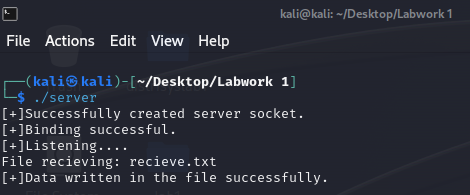
\includegraphics[scale=1.0]{images/server.PNG}
    \caption{Server side}
\end{figure}

\end{document}

\end{document}